\begin{figure}[t]
    \centering
    \begin{subfigure}[b]{0.5\linewidth}
        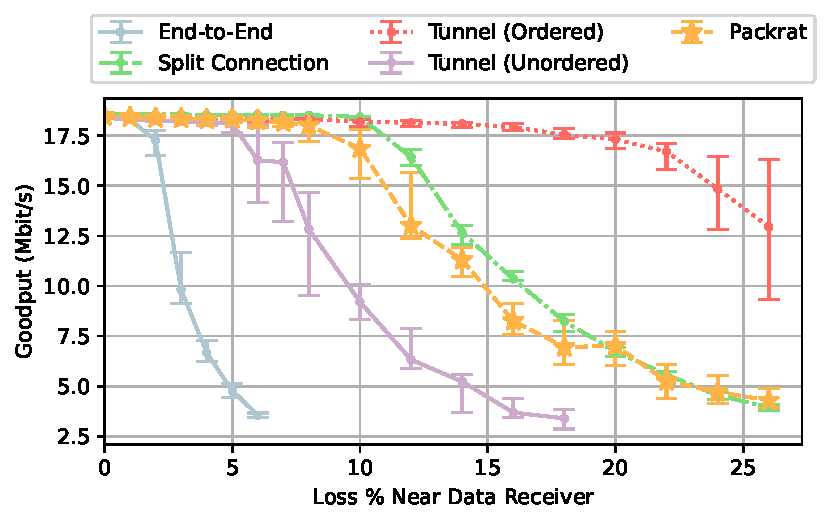
\includegraphics[width=\linewidth]{packrat/figures/http_benchmark.pdf}
        \caption{QUIC HTTP/3 file download.}
        \label{fig:packrat:perf:http}
    \end{subfigure}
    \begin{subfigure}[b]{0.48\linewidth}
        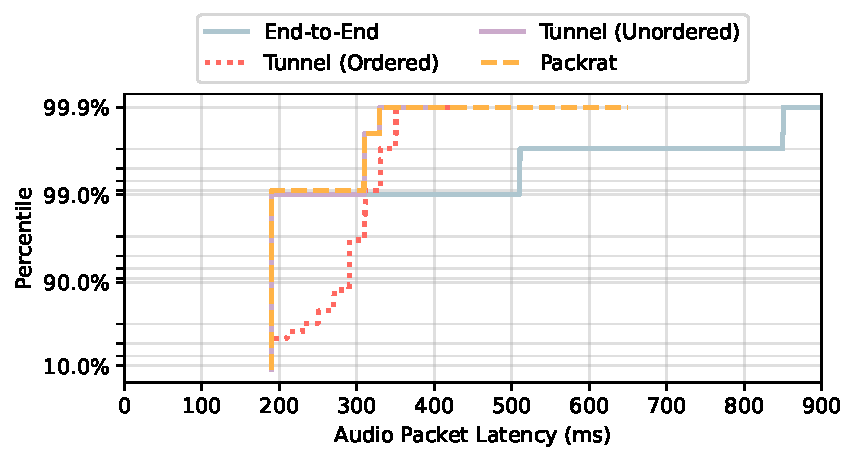
\includegraphics[width=\linewidth]{packrat/figures/media_benchmark.pdf}
        \caption{Low-latency media stream with FEC.}
        \label{fig:packrat:perf:media}
    \end{subfigure}
    \begin{subfigure}[b]{0.48\linewidth}
        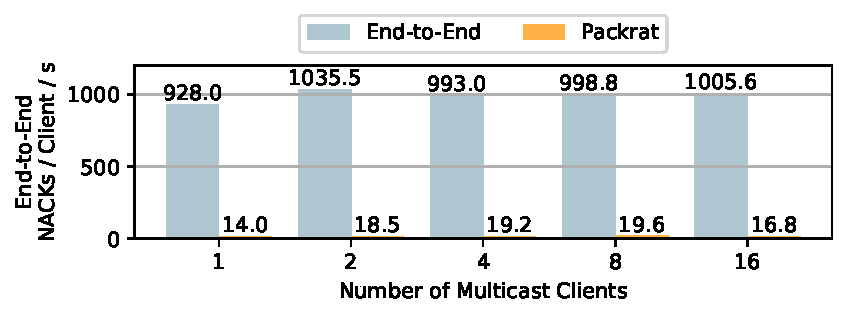
\includegraphics[width=\linewidth]{packrat/figures/multicast_benchmark.pdf}
        \caption{Reliable IP multicast stream.}
        \label{fig:packrat:perf:multicast}
    \end{subfigure}
    \caption{In-network retransmissions from the Packrat proxy enable applications
     to achieve better throughput, latency, and link
     overheads in lossy network settings compared to end-to-end
     retransmissions. Applications using the tunnel differ in whether they
     benefit based on the tunnel configuration, which is a disadvantage of
     link-layer retransmissions.}
    \label{fig:packrat:perf}
\end{figure}